\section{Medien}
\subsection{Ausbreitungsgeschwindigkeit}

Lichtgeschwindigkeit im Vakuum: $c_0 = 299'792'458 \frac{m}{s}$ \\
Faustregel in Medien: $200'000 \frac{km}{s} = 20 \frac{cm}{ns}$

\subsection{Signaldämpfung}
\small{Angegeben in Dezibel; auch: Insertion Loss, Attenuation}

Dämpfung $A =  10 * \log(P_1 / P_2) = 20 * \log(U_1 / U_2)$

Höhere Frequenz $\rightarrow$ mehr Dämpfung

\textcolor{orange}{Halbierung der Leistung entspricht ca. 3dB}

\subsubsection{Signal-to-Noise-Ratio SNR}

$ SNR = 10 * \log(P_{Signal} / P_{Noise}) dB $

\subsection{Kabel}

\subsubsection{Koaxial}
\begin{minipage}{0.5\linewidth}
    \begin{itemize}
        \item[+] besser als twisted pair für hohe Frequenzen
        \item[+] relativ unempfindlich gegen elektromagn. Störungen
        \item[-] mechanisch heikel (knicken/quetschen)
    \end{itemize}
\end{minipage}
\hfill
\begin{minipage}{0.4\linewidth}
    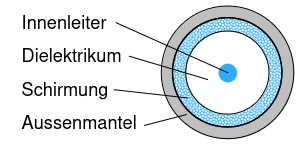
\includegraphics[width=\linewidth]{koax-quer}
\end{minipage}


\subsubsection{Parasymmetrisch (Twisted Pair)}
\begin{itemize}
    \item[+] bereits lange im Einsatz
    \item[+] bei guter Qualität auch für Breitband geignet
    \item[-] mit oder ohne Schild
\end{itemize}

\subsubsection{Shielded Twisted Pair (STP)}

Bezeichnet nach ISO 11801: \textcolor{orange}{xx}/\textcolor{blue}{y}TP

\begin{multicols}{2}
    \textcolor{orange}{xx} steht für die Gesamtschirmung
    \begin{itemize}
        \item[U] ungeschirmt
        \item[F] Folienschirm
        \item[S] Geflechtschirm
        \item[SF] Folien- \& Geflechtschirm
    \end{itemize}

    \columnbreak

    \textcolor{blue}{y} steht für die Aderpaarschirmung
    \begin{itemize}
        \item[U] ungeschirmt
        \item[F] Folienschirm
        \item[S] Geflechtschirm
		\item[\vspace{\fill}]
    \end{itemize}
\end{multicols}


\subsubsection{Störungen bei TP}

Kapazitive/Induktive Störungen treten bei TP öfter als bei Koax oder Glasfaser auf.

Kapazitive Störungen von benachbarten Leitungen heissen Crosstalk(über-/nebensprechen).
Diese Störungen können durch ein invertiertes komplementäres Signal weitgehen aufgehoben werden.
Der Empfänger subtrahiert die beiden Signale und eliminiert dadurch Störungen.

\begin{center}
    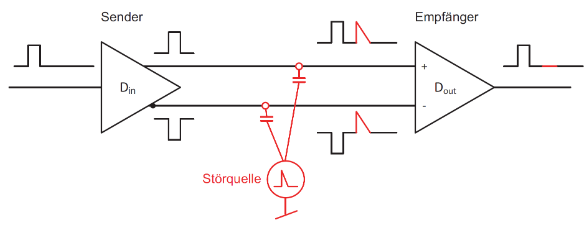
\includegraphics[width=0.8\linewidth]{tp-stör-komplementär}
\end{center}

Alternativ können kapazitive Störungen mit einem leitenden Schirm abgefangen werden.

\begin{center}
    \includegraphics[width=0.8\linewidth]{tp-stör-schirm}
\end{center}

Induktive Störungen (durch ein Magnetfeld) können nicht durch ein komplementäres Signal alleine gelöst werden, da
die die Störung auf beiden Signalen entgegengesetz ist.
Dies kann über verdrillen der Adernpaare gelöst werden, benachbarte Schleifen heben sich
so immer auf.

\begin{center}
    \includegraphics[width=0.8\linewidth]{tp-stör-twist}
\end{center}


\subsection{Kategorien}

\begin{center}
    \begin{tabular}{@{$\bullet \,$}ll}
        Cat 1..4 & Billigkabel für analoge Sprachübertragung (< 1Mb/s)     \\
        Cat 5    & bis 100 MHz, z.B. 100Mb/s oder 1 Gb/s Ethernet bis 100m \\
        Cat 6    & 250 MHz, 1 Gb/s Ethernet und 10 Gb/s Ethernet bis 55m   \\
        Cat 7    & 600 MHz, z.B. für 10 Gb/s Ethernet bis 100m             \\
    \end{tabular}
\end{center}


\subsection{Lichtwellenleiter}

\begin{itemize}
    \item[+] hohe Bandbreite $\rightarrow$ hohe Datenrate
    \item[+] geringe Dämpfung $\rightarrow$ lange übertragungsstrecken
    \item[+] resistentt gegen elektromagnetische Störungen
\end{itemize}

Zentrum aus Kernglas mit hoher optischer Dichte (Brechungsindex $n_{kern} = 1.5$)
umschlossen von Mantelglas mir geringer optischer Dichte (Brechungsindex $n_{mantel} = 1.48$).
Dadurch werden Lichtstrahlen im Kern totalreflektiert($\beta > 90 \degree$) und keine Energie durch Absorption
verloren

\subsubsection{Multimode}
\begin{itemize}
    \item[+] dicker Kern (mehrere Wege/Modes für das Licht)
    \item hohe Dispersion(Signalverschmierung auf langen Wegen)
    \begin{itemize}
        \item Kann reduziert werden durch Einsatz von Gradientenfaser (übergang zwischen
            Kern und Mantel)
    \end{itemize}
\end{itemize}

\subsubsection{Singlemode}
\begin{itemize}
    \item[+] keine Dispersion
    \item[+] hohe Datenraten auf hohe Distanzen
    \item dünner Kern, nur eine Grundmode
\end{itemize}



